\documentclass[12pt]{article}
\usepackage[right=0.7in,left=0.7in,top=1in,bottom=1in]{geometry}
\usepackage{hyperref}
\hypersetup{colorlinks, citecolor=blue, filecolor=blue, linkcolor=blue, urlcolor=blue}
\usepackage{graphicx}
\usepackage{url}
\usepackage[round]{natbib}
\usepackage{amsmath,amsthm}
\usepackage{engord}
\usepackage{float}
\usepackage{subfig}
\usepackage{pdflscape}
\usepackage{booktabs}
\usepackage{pgfplots}
\usepackage{subfig}
\pgfplotsset{compat=1.14}
\usepackage{longtable}
\pgfplotsset{every axis label/.append style={font=\tiny}}
\usepackage[labelsep=period]{caption} %% This switches "Table 1: Title" to "Table 1. Title"
\usepackage{authblk}
\usepackage{amssymb} %% Necessary, just for the \checkmark command  in tables.
\usepackage{multirow} %% Necessary if we are doing tables in LaTeX

\usepackage{xr}

\usepackage{setspace}
\doublespacing

\usepackage{sectsty}
\sectionfont{\large}
\subsectionfont{\normalsize}
\subsubsectionfont{\normalsize}

\newcommand{\specialcell}[2][c]{\begin{tabular}[#1]{@{}l@{}}#2\end{tabular}}

%%%%%%%%%%%%%%%%%%%%%%%%%%%%%%%%%%%%%%%%%%%%%%%%%%%%%%%%%%%%%

\title{ \vspace*{-2.5cm} \hspace*{-0.5cm}Evaluating the Impact of Offline Store Clusters in the Age of Platforms: Evidence from China's Metropolitan Real Estate Market \footnote{
The preliminary version was entitled "Property brokerage, Partial monopoly and Housing market" and was presented at The 1st Summer Meeting in Urban Economics, China. We are grateful for the comments and suggestions made at the meeting. The code to replicate the paper can be accessed at \href{https://github.com/sergiozxy/RealEstateBrokerage}{https://github.com/sergiozxy/RealEstateBrokerage} The authors gratefully acknowledge financial support from the Fundamental Research Funds for the Central Universities of Sichuan University (2019hhf-08; SKSYL201812; 2018jj-01) and National Natural Science Foundation of China (71773081). We gratefully thank for Hanying Liu from Sichuan University and Chongyu Wang from Florida State University for insightful feedback.
}}


\date{ \vspace*{0.5cm} \today}

%%%%%%%%%%%%%%%%%%%%%%%%%%%%%%%%%%%%%%%%%%%%%%%%%%%%%%%%%%%%%

\begin{document}


\author[1]{Guoying Deng}
\author[2]{Xuyuan Zhang \thanks{Email Address: \href{mailto:zxuyuan@umich.edu}{zxuyuan@umich.edu}}}
\affil[1]{Sichuan University}
\affil[2]{University of Michigan, Ann Arbor}

\bgroup
\let\footnoterule\relax

\begin{singlespace}
\maketitle

% Police brutality, law enforcement, and crime: Evidence from Chicago
\begin{abstract}
    \noindent This study examines the impact of offline store expansion by Lianjia, China's leading real estate brokerage, in the context of online platform development. By analyzing micro-level transactions of second-hand houses in ten major Chinese cities from 2016 to 2022, the study explores how the strategic clustering of offline stores enhances Lianjia's influence in local communities and facilitates the creation of an extensive franchise network. This study first conducts a regression discontinuity (RD) design to quantify the optimal influence radius of these stores on housing transactions. By incorporating the optimal influence radius, this study examines the exogenous shock of Lianjia's market entry to identify a significant increase in transaction revenues. However, this effect is diminished during Covid-19 periods. In addition, the paper examines the impact of Lianjia's ACN strategy on its platformization efforts and concludes that the effect is not only from the larger client base brought by the platform, but also from the information control by sharing information within the platform. This study provides valuable insights into the synergy between offline store expansion and online platform development, highlighting their importance in the evolving real estate brokerage market.
  \end{abstract}
  
  \textbf{Keyword}: Marketing Strategy, Housing Markets, Digital Platforms
  
  \textbf{JEL} Classification Codes: D4, L1, L8, R3
\end{singlespace}
\thispagestyle{empty}

\clearpage
\egroup
\setcounter{page}{1}

%% Temporary tool to track how this paper is structured. Feel free to comment in or out. 
% \tableofcontents
% \bigskip

%%%%%%%%%%%%%%%%%%%%%%%%%%%%%%%%%%%%%%%%%%%%%%%%%%%%%%%%%%%%%
%%%%\section{Introduction\label{sec:introduction}}

\section{Introduction \label{sec:introduction}}

\noindent

In the real estate market, transaction cost is a critical factor for both buyers and sellers. Minimizing these costs has made the selection of competent real estate agencies a significant priority for both parties. Especially in the context of China's burgeoning real estate market, brokerage firms are assuming an increasingly important role in facilitating the communication channel between buyers and sellers \citep{glaeser_real_2017}. In addition, technological advancements coupled with the proliferation of dominant platforms have created a trend toward greater monopolization within the real estate brokerage industry, rather than fostering a competitive environment. Therefore, it is imperative to analytically examine the expansion strategies of Chinese real estate agencies, especially in the context of escalating platform-based monopolization.

Lianjia is the largest real estate brokerage in China that has platformed real estate transactions by establishing the Beke platform. They can expand rapidly by the expansion of offline stores on a large scale while sharing resources by leveraging the advantages of their platform. Beke has also established an original Agent Cooperate Network (ACN) that integrates and shares the content of its multiple subsidiaries to realize multiple revenue models at the same time.\footnote{The ACN model breaks down the entire process of transaction into parts, each of which is handled by a single person or store, including seller-side: finding sellers, maintaining the listing of the house, commissioning and communicating, and buyer-side: Finding clients, matching homes and clients, facilitating transactions, and providing financial services assistance.} Through the ACN model, Lianjia transforms the internal competition within the system into the overall competitiveness of the system, improving the reputation and influence of the entire brand and gaining a more favorable position in the marketplace. For example, according to the data of AutoNavi Map and CREIS data: In 2020, the number of real estate agent stores in the main urban area of Chengdu City that accessed Beke Housing's platform accounted for about 20\%, but the market share reached 73.98\%.

The reason why Lianjia does not have such a high proportion of offline stores in the market but has an absolute dominant position in metropolis can be explained by the mechanism of China's second-hand real estate market. In the China's real estate market, brokerages still operate on a bilateral agency model, where sellers need to choose the agency that can help them sell their home in the fastest time and for the highest price possible for the transaction. However, due to the asymmetric information characteristics of the real estate market, sellers must find a way to inform buyers and match buyers. In a fully competitive market, sellers would be indifferent in choosing real estate agents.  Nevertheless, as the market trends towards increased monopolization, sellers encounter a dichotomous choice: opt for a larger brokerage firm, which, albeit commanding higher fees, possesses the capacity to expedite housing transactions, or engage with a smaller brokerage, which presents a contrasting scenario of lower fees yet potentially less efficient transaction facilitation.

While it is possible for sellers to adopt a multi-homing strategy, this approach is suboptimal for several reasons. First, the exclusivity of contracts between sellers and agents precludes the adoption of a multi-homing strategy. Second, although sellers can list their houses with multiple brokerages, smaller brokerages often lack a broad enough target client base, which is not very helpful in selling the homes. Third, connecting with multiple brokers simultaneously can make each brokers feel that they are in a difficult position to compete for that house, which reduces their incentive to be proactive in their efforts. Finally, while the variance in service costs between agencies is acknowledged, these costs are trivial compared to the value of the property and are more related to the risk associated with holding a financial asset. Consequently, risk-averse individuals are inclined to choose an agency that provides a guaranteed level of service. Due to the mechanism of online promotion and offline transaction in the real estate brokerage industry, the nature of the brokerage's services in the offline stores is of high value for its influence on the client side. This is the principle behind Lianjia's choice to open stores in the neighborhoods of each target community. By opening a wide range of stores around the communities, the brokerage attracts sellers to list their houses, and attracts buyers in the market through its extensive platform sources, thus obtaining a higher number of transaction and income from the transaction.

In this paper, we empirically test this hypothesis that when brokerages are able to expand their offline stores' coverage in the communities, the brokerages can earn higher income in this community, and we decompose the channels into two parts. On the one hand, is that when brokers have better control over listing information by opening additional offline stores, they are more likely to attract more sellers to choose them, which will then benefited by the online platform effect to extract more buyers and more likely to complete a transaction. On the other hand, when offline stores are closer to the communities, they are more likely to make a house tour to help the buyers to get more information on the house, and therefore, be more likely to complete a transaction. During the Covid-19 pandemic period, the Chinese government restricts the number, and in this period, we find that the number of houses tour is not significantly affected by the number of offline stores, but the listing information significantly decreases because the brokerages are difficult to interact with the sellers and then failure to maintain the information advantage during this period.

Apart from directly measuring the dynamic effect of Lianjia's offline stores to transaction, we use Lianjia's entry into the local segmented market as an exogenous shock to test the effect of entry on transaction characteristics. The results indicate that when Lianjia enters the market, revenues increase significantly, but this is not due to the larger clinic-based, but due to the greater information control brought by the newly opened store. Moreover, during pandemic periods, we find that all effects are diminished, meaning that during pandemic periods, both the client-based effect and the housing information are diminished. Simultaneously, our study also examines the impact of Lianjia's ACN strategy on the real estate market, focusing on its effect on offline store operations. Through this exogenous shock, we find that post-2018, the ACN significantly boosts revenue and alters consumer behaviors, especially in terms of price concessions and house tours. Also, contrary to the previous effect, the effects are diminished during pandemic periods. The findings highlight the resilience of physical stores during a global epidemic and underscore the necessity for a synergistic evolution of online and offline strategies.

The remainder of the paper proceeds as follows. Section \ref{sec:literature_review} reviews the literature that is related to our research. Section \ref{sec:data} describes the data and summarizes the statistical evidence. Section \ref{sec:mechanism_design} presents the main result of our finding. Finally, Section \ref{sec:conclusion} concludes. 


\section{Literature Review} \label{sec:literature_review}

\citet{Rosen_hedonic} proposed a hedonic pricing model and explained the price is determined by internal and external factors affecting it. But the hedonic pricing model suffers under conditions of market asymmetry and information inequality. The seminal work on the impact of asymmetric information in markets is \citep{Akerlof_1970}, which demonstrated that markets for used cars tend to be dominated by low-quality goods, or 'lemons,' leading to market inefficiencies.  Furthermore, \citet{grossman_impossibility_1980} further argued that information effective market assumption is hard to hold in reality. Therefore, the real estate market, which is characterized by information asymmetry, is particularly vulnerable to the adverse selection problem. In this context, the role of real estate brokerages is crucial, as they act as intermediaries between buyers and sellers, providing valuable information and facilitating transactions.

In terms of real estate market, several literature has shown that several factors can influence the market pricing and strategies. The \citep{550a6ccf-cde2-3dd1-979f-1a8db2b8ceb9} documents that apart from price competition in the market, there is a lot of market inefficiency that stems from non-price competition, which suggests that as the degree of competition in the market increases, the market becomes progressively less efficient, indicating that the entry dividend begins to fall and aggregate social welfare begins to decline. Moreover, \citet{hendel_relative_2009} analyzes two types of listings in the second-hand housing market and finds that For-Sale-By-Owner type of platforms are less effective in terms of time and probability of sale, while operating better compared to listing homes for sale as a broker. In addition, \citet{bailey_economic_2018} uses data from the social media site Facebook to show that social interactions can influence people's economic decisions. Their results show that people who have friends who are geographically distant in real life and who have a hunch that house prices are about to rise are more likely to buy a house than rent one. Other relevant areas of research include \citep{NIEUWERBURGH_information, salz_intermediation_2022}.

With respect to the behavior of real estate brokerages, the research conducted by \citep{AGARWAL2019715} substantiates that these entities, acting as intermediaries in market transactions, possess superior knowledge of market dynamics. This informational superiority enables the intermediaries to use their bargaining power to secure discounts in the market. Similarly, \citet{HAN2015813} articulates that brokerages operating in unidirectional and bidirectional markets exhibit different levels of bargaining leverage, leading to different motivational drivers. This mechanism is in line with other research, which shows that properties with lower commission rates have a 5\% less likelihood of being sold and takes 12\% longer to sell \citep{10.1257/app.20160214}.

Regarding the impact of online platforms on the real estate sector, research by \citep{ZUMPANO2003134} suggests that while the length of time buyers spend searching for properties remains unchanged, the scope of their search expands to include a greater number of online listings. \citet{ZHANG2021101104} show that the introduction of online platforms is associated with reductions in existing home prices and increased sales volumes, effects that are influenced by new home prices and household size. However, a comprehensive analysis of the influence of the physical stores of online platforms on the real estate market is still lacking in the literature. 

Finally, the impact of real estate intermediaries on the market can be decomposed into several aspects. Using a model based on the assumption of a perfectly competitive market in which an influx of brokers competitively enters the market, \citet{williams_agency_1998} shows that the presence of brokers in the market equilibrium exceeds the optimal number of allocations, thereby causing a reduction in social welfare. Moreover, the results show that neither brokers nor sellers are motivated to deviate from the equilibrium price structure, which coincides with the reservation price set by sellers. Complementary research in another study shows that a significant influx of brokers into the market is correlated with a decrease, rather than an increase, in house prices, along with a gradual decrease in transaction cycles within the market \citep{https://doi.org/10.1002/jae.2891}. Furthermore, the work of \citep{qu_identifying_2021-1} highlights the moderating role of broker commissions on the dissemination of market information during transactions. Their findings suggest that the use of a broker can significantly mitigate the concessions that sellers are forced to make in the transaction process, thereby enhancing their ability to complete a home sale more efficiently.


% 由于房地产中介行业线上推广线下成交的机制,中介机构在线下门店中的服务性质对于其在客源方的影响具有很高的价值。链家通常选择在每个目标小区的周边开店便是该原理。链家通过在小区周边大范围开店,从而吸引卖方选择该机构进行挂牌,而又通过其广泛的平台客源来吸引市场中的买方从而获得更多的成交数量与成交收入。由于房地产中介行业线上推广线下成交的机制,中介机构在线下门店中的服务性质对于其在客源方的影响具有很高的价值。链家通常选择在每个目标小区的周边开店便是该原理。链家通过在小区周边大范围开店,从而吸引卖方选择该机构进行挂牌,而又通过其广泛的平台客源来吸引市场中的买方从而获得更多的成交数量与成交收入。


\section{Data and Descriptive Evidence \label{sec:data}}

\subsection{Data Collection and Processing}

This study focuses on the housing markets in ten major cities in China, namely Beijing, Shanghai, Chongqing, Tianjin, Shenzhen, Guangzhou, Chengdu, Hangzhou, Wuhan and Nanjing. These cities are not only central to China's economic development, but also reflect the broader trends and characteristics of the country's real estate dynamics. Spanning from 2016 to 2022, the research period encapsulates a pivotal era in China's real estate sector. During the first phase of the study, from 2016 to 2019, the housing markets in these cities experienced a remarkable boom. This period was characterized by significant growth in property prices, supported by robust economic expansion and increased demand in these urban centers. However, the final phase of our study, from 2020 to 2022, paints a contrasting picture. During this period, China's overall economic growth rate has been slower significantly, which has also reflected in a slowdown in the real estate markets of these major cities. In addition, the Chinese government has implemented strict rules in Covid-19 protection, so the real estate agents in these major cities are significantly affected.

The second hand housing transaction data was collected form \href{https://bj.lianjia.com/}{lianjia.com} for ten cities ranging from 2016 to 2022. Initially, we filtered out transaction records exhibiting unusually high prices, identifying them as outliers that could skew the analysis. We then removed records with missing values to maintain the integrity of our dataset. We also removed any records that were listed duplicated. We finally have a data with length 1,716,579 second-hand house.\footnote{Due to government restrictions, four of these cities did not list the transaction price for each transaction during the study period.} Since most of the offline stores in lianjia are community-based, and most of the information is accurate at the community level, we decided to aggregate the information at the community level to make our panel compatible. By taking the average of all transaction information, we constructed the panel data with seven years.

To gather other characteristics information, we first extracted the POI data from the AutoNavi map using the web-scrawling Python program.\footnote{AutoNavi, a leading mapping application in China with a huge user base of more than 700 million, stands out for its detailed and accurate POI data and precise public transportation information. These features underscore AutoNavi's formidable lead in the digital mapping sector, highlighting its ability to provide unparalleled navigation accuracy and comprehensive urban mobility solutions. Our extracted AutoNavi map contains more than 1 million POIs for each city in each year.} We then classified the extracted POIs into different categories, the specifics of which are discussed in detail in Table \ref{tab:statistical}. This categorization was crucial for understanding the urban infrastructure and amenities available in the vicinity of the analyzed properties. We prioritized POIs within a 500-meter radius-a distance typically covered within a ten-minute walk, consistent with urban planning standards for accessible urban design. This radius was specifically chosen to reflect the immediate urban environment that influences residential desirability and value, as the majority of these POIs provide recreational services. Furthermore, some geo-informational data was also integrated into our research data, which consists of the annual gdp obtained from \citep{zhao_forecasting_2017}, nighttime lights data, obtained from \citep{elvidge_annual_2021} and air pollution data from \citep{doi:10.1021/acs.est.1c05309}. By merging these data with our research panel, we finally get the data.


\subsection{Influential Radius} \label{subsec:Influential_Radius}

The effectiveness of an offline intermediary's influence on its immediate communities is inherently constrained by geographic limitations, with its influence decreasing in proportion to the increase in spatial distance. Moreover, since the offline stores of lianjia are directly operated by the company, strategic considerations regarding the optimal distance between stores are an integral part of their location planning to mitigate the risks associated with over-concentration of stores that could lead to competitive overlap and service homogenization. Consequently, it is imperative to determine an optimal radius threshold and subsequently assess the diversity of agencies operating within this demarcated zone.

To determine the optimal radius of influence, this research employs a regression discontinuity design (RDD) method to examine the influential radius of offline real estate brokerages. The dependent variable in this analysis is the transaction revenue generated by Lianjia within a given community, while the independent variable is the community's proximity to the nearest Lianjia's store. Given that stores are predominantly located within commercial districts-typically encompassing several streets no more than two kilometers in diameter-it is assumed that a requisite number of stores within each district is essential to sustain revenue generation in that community. In addition, since the Lianjia's company adopts a 5-minute walking distance (approximately 400 meters) radius policy, which means that no matter how far away customers live, they should be accessible within a 5-minute walk to the nearest Lianjia's store. Building on this premise, the study further investigates the existence of an optimal influence radius within shopping districts, defined as the distance radius within which the presence of a Lianjia optimally increases transaction revenues. At the same time, the study also examines the hypothesis that beyond this optimal radius, the impact on transaction revenues diminishes as a result of the strategic store layout decisions implemented by Lianjia.

\begin{figure}[ht]
    \centering
    \subfloat[RD plot with first order polynomial]{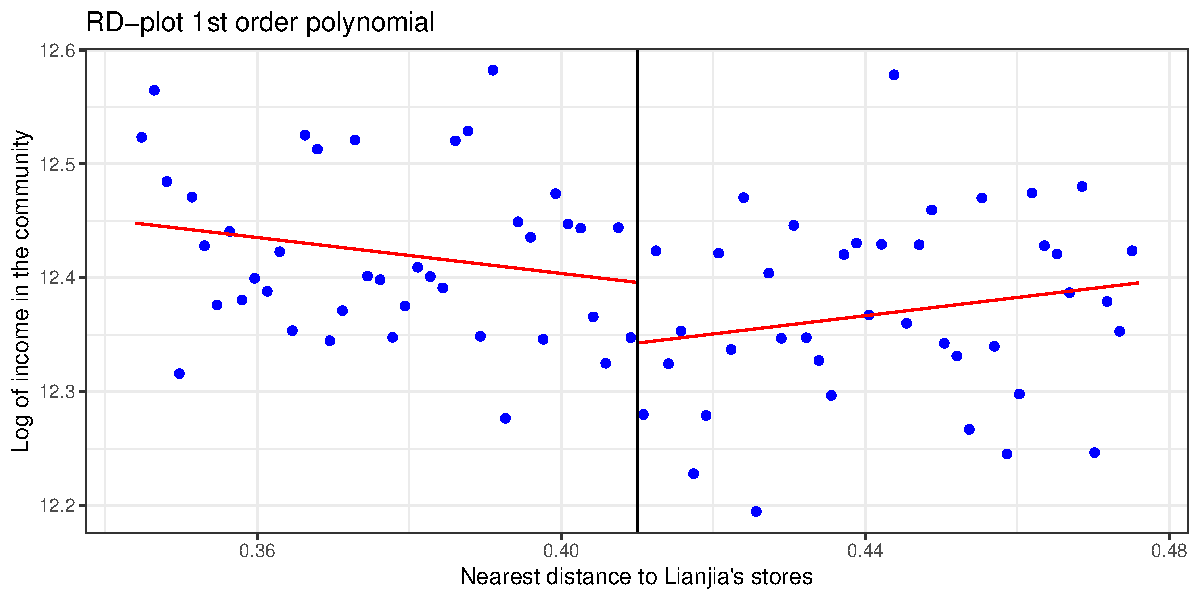
\includegraphics[width=0.5\textwidth]{../figures/RD_Plot_1st_Order.pdf}\label{fig:RD_Plot_1st_Order}}
    \hfill % Adds horizontal space between figures
    \subfloat[RD plot with second order polynomial]{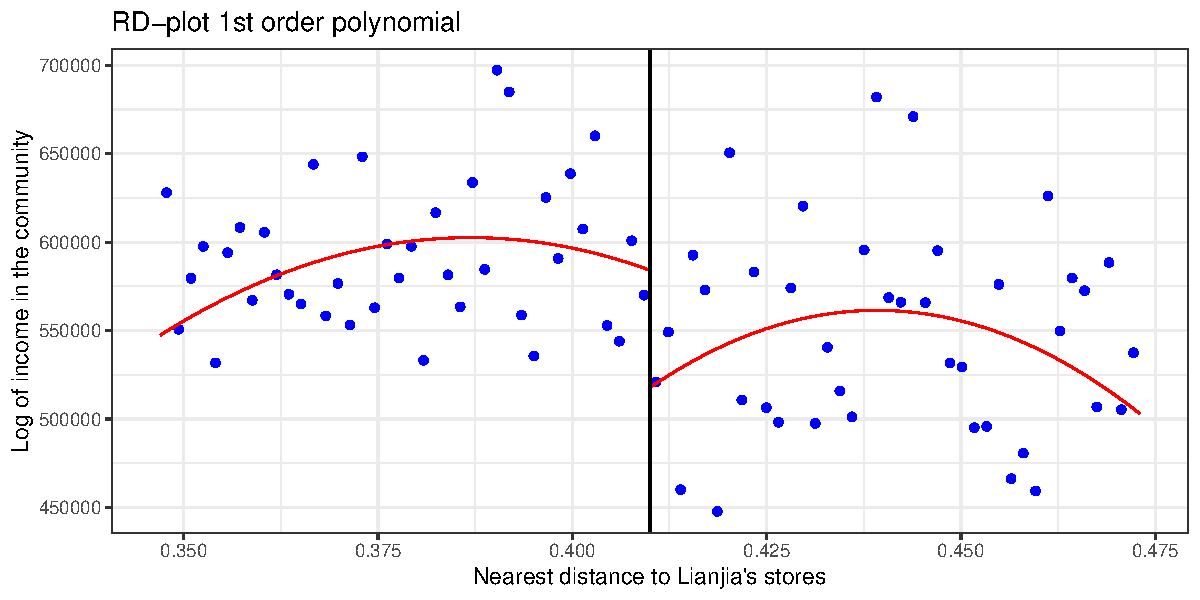
\includegraphics[width=0.5\textwidth]{../figures/RD_Plot_2nd_Order.pdf}\label{fig:RD_Plot_2nd_Order}}
    \hfill % Adds horizontal space between figures
    \subfloat[RD plot with third order polynomial]{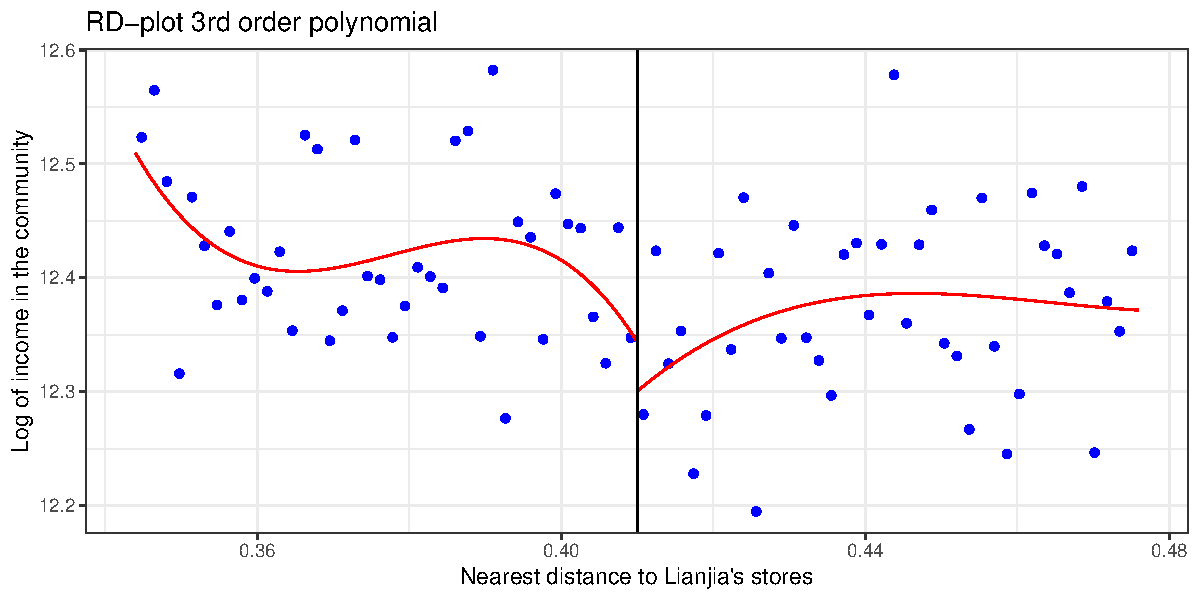
\includegraphics[width=0.5\textwidth]{../figures/RD_Plot_3rd_Order.pdf}\label{fig:RD_Plot_3rd_Order}}
    \caption{RD design}
    \label{fig:RD_design}
\end{figure}

From Figure \ref{fig:RD_design} we can see that there is indeed discontinuity in 410 meters of communities to the nearest Lianjia's store, which is pretty close to the lianjia's 5-minute walk distance policy. The observed decline in the Lianjia's influence is marked and suggests a pronounced reduction in its impact on the system overall within our study sample. This phenomenon can be attributed to the implementation of the Lianjia's proximity to customers policy, which is evidenced at the data level. 

To make the robust check we conducted Donut Hole test by excluding observations close to the cutoff and estimating the effect with the remaining data. The results are shown in Appendix and the result shows that the discontinuity still exists and this provides evidence against a model misspecification. Furthermore, we carry out the density test by \citep{MCCRARY2008698}. The result shows that the p-value is greater than 0.1, which suggests the result is not due to manipulation of polygons. Finally, we carry out placebo tests which are reported in Appendix, which strengthens the case for a true treatment effect.

\subsection{Statistical Summary}

After constructing our optimal radius, we recalcualte the number of lianjia and other brokerages' stores within this radius. To check the robustness of the data, we divide our data to those with lianjia and those without lianjia and to check whether lianjia's offline stores have influential effect on the transaction effect in the community. We can see that for income, house tour number and the are all significantly different in those communities with or without lianjia. Furthermore, we find that the other brokerages are also have the same tendency that they typically open stores with the same strategy as lianjia, which is consistent with our Theoretical Model's Proposition [xxxxx]. This figure is shown in Figure \ref{fig:same_distribu`tion}.
`'
\begin{table}[htb!]
    \centering
    \begin{tiny}
    \caption{Statistical Summary}
    \begin{tabular}{p{5cm}lllll}
\toprule
Name & Mean without lianjia & SD without lianjia & Mean with lianjia & SD with lianjia & Difference \\
\midrule
The time it takes before a deal is made. & 13.59 & 14.56 & 17.09 & 17.50 & -3.501 (-49.823***) \\
price\_concession & -0.0367 & 0.0318 & -0.0351 & 0.0294 & -0.00200 (-12.088***) \\
percentage of lianjia to all brokerages & 0 & 0 & 0.206 & 0.166 & -0.206 (-384.429***) \\
number of brokerages within 410 meters, which is the cutoff of RD & 5.362 & 6.871 & 12.66 & 8.410 & -7.300 (-217.614***) \\
The number of people watching a listing. & 17.61 & 29.11 & 20.29 & 29.40 & -2.682 (-21.214***) \\
The final agreed price. & 260.5 & 254.9 & 351.9 & 292.1 & -91.48 (-76.662***) \\
without online platformization influence & 0.195 & 0.396 & 0.233 & 0.423 & -0.0380 (-21.384***) \\
The number of times a listing is watched. & 1121 & 1827 & 1233 & 1969 & -112.4 (-13.636***) \\
The number of times a negotiation was held. & 4.769 & 7.686 & 5.683 & 10.78 & -0.914 (-22.178***) \\
The period over which negotiations took place. & 150.5 & 187.5 & 166.6 & 239.1 & -16.06 (-17.075***) \\
Referring to electronic shops. & 1.489 & 3.566 & 1.942 & 4.365 & -0.453 (-26.004***) \\
Referring to proximity to kindergartens & 8.665 & 6.229 & 11.76 & 6.081 & -3.097 (-116.630***) \\
Referring to proximity to hotels & 3.211 & 5.287 & 5.428 & 6.315 & -2.217 (-87.264***) \\
Referring to shopping mall. & 4.554 & 7.539 & 6.698 & 8.489 & -2.144 (-61.405***) \\
Distance to the nearest museum. & 0.617 & 1.533 & 1.023 & 1.869 & -0.406 (-54.395***) \\
Referring to old care systems. & 0.894 & 1.628 & 1.339 & 1.950 & -0.446 (-56.870***) \\
Referring to KTV and some entertainment venues. & 5.179 & 7.853 & 7.305 & 7.759 & -2.126 (-63.096***) \\
Referring to middle schools. & 2.059 & 2.329 & 3.368 & 2.853 & -1.309 (-115.077***) \\
Referring to primary schools. & 2.812 & 2.846 & 4.343 & 3.205 & -1.531 (-116.172***) \\
Referring to the availability of western food nearby. & 3.880 & 7.709 & 7.317 & 10.02 & -3.437 (-87.756***) \\
Referring to proximity to supermarkets (measured by number within given distance & 3.155 & 3.374 & 4.499 & 3.686 & -1.344 (-87.586***) \\
Referring to proximity to subway stations. & 0.683 & 0.945 & 1.111 & 1.099 & -0.429 (-96.038***) \\
Referring to parks. & 3.422 & 4.575 & 4.569 & 3.944 & -1.147 (-62.708***) \\
The area of a property. & 90.82 & 48.57 & 84.97 & 39.15 & 5.845 (31.050***) \\
The number of bedrooms in a property. & 2.338 & 0.816 & 2.202 & 0.730 & 0.136 (40.958***) \\
The number of toilets in a property. & 1.306 & 0.579 & 1.246 & 0.455 & 0.0600 (26.915***) \\
The age of the house. & 18.08 & 11.68 & 20.73 & 11.77 & -2.651 (-52.316***) \\
The level on which a particular room or apartment is, within a building. & 1.854 & 0.975 & 1.933 & 0.931 & -0.0790 (-19.324***) \\
The ratio of the green space to the total plot area. & 0.309 & 0.237 & 0.300 & 0.107 & 0.00900 (12.288***) \\
The total number of buildings in an area. & 26.88 & 56.66 & 20.51 & 50.54 & 6.371 (27.653***) \\
The number of floors in a building. & 12.75 & 8.454 & 12.97 & 8.485 & -0.221 (-6.035***) \\
The number of living rooms in a property. & 1.445 & 0.504 & 1.341 & 0.492 & 0.104 (48.345***) \\
The ratio of elevators to the total number of floors. & 0.453 & 0.413 & 0.408 & 0.279 & 0.0450 (30.475***) \\
The number of kitchens in a property. & 0.983 & 0.150 & 0.983 & 0.125 & 0 (-0.459) \\
The ratio of the floor area to the total plot area. & 4.942 & 329.1 & 2.702 & 9.385 & 2.240 (2.367**) \\
The total number of residents in an area. & 995.8 & 1079 & 901.8 & 956.5 & 93.97 (21.484***) \\
Air quality measure. & 44.08 & 13.29 & 45.74 & 13.89 & -1.664 (-28.266***) \\
Population density. & 15506 & 16336 & 24634 & 18866 & -9100 (-118.769***) \\
Night time lights. & 32.62 & 13.59 & 38.41 & 11.92 & -5.782 (-105.485***) \\
\bottomrule
\end{tabular}

    \label{tab:statistical}
    \end{tiny}
\end{table}

\begin{figure}
    \centering
    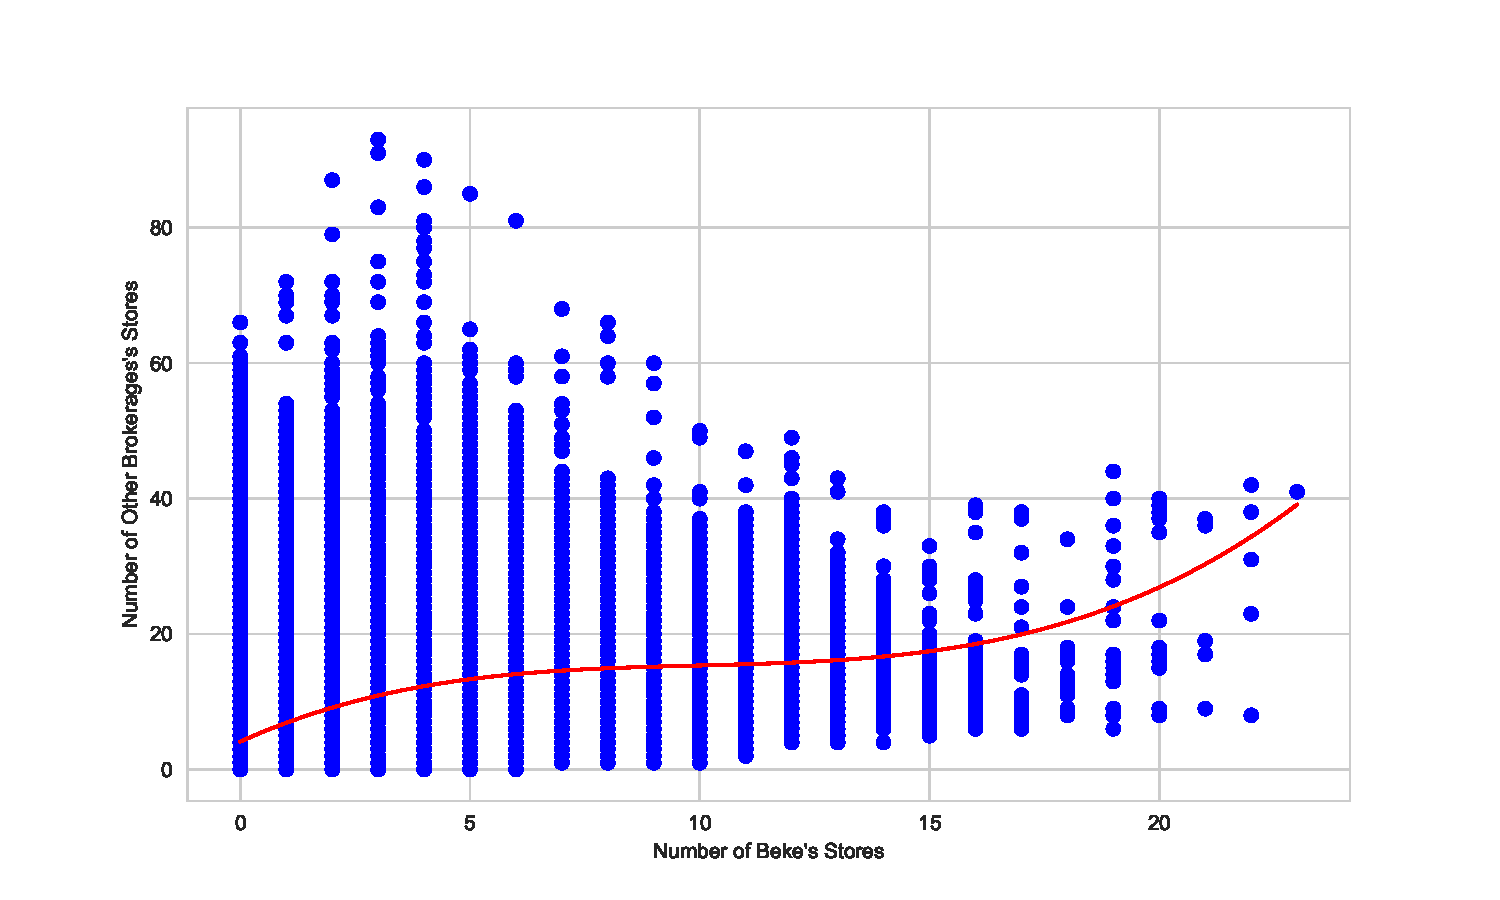
\includegraphics[width=0.7\textwidth]{../figures/scatter_plot_with_two_brokerages.pdf}
    \caption{Tendency between two types of brokerages}
    \label{fig:same_distribution}
\end{figure}


\section{Theoretical Model}

To characterize the real estate brokerage market, we can assume that there are two types of brokerages in the market, where the type $1$ denote the large real estate brokerage that is incorporating the online platform and the offline stores strategies, and the type $2$ denote the small real estate brokerage that only have the offline stores and they should compete with the type $1$ stores and type $2$ stores in the market. Each type of brokerage follows a standard percentage charge by $r_j$ and they can not manipulate the percentage charge in each submarket.

We can assume that there are $M$ number of communities in the market, and each market has $\kappa_i, i \in \{1, \ldots, M\}$ number of houses listed which depends on the previous listing number and we can formulate it as a AR(1) model specified by:

\begin{equation}
  \kappa_{i, t} = \rho_{i} \kappa_{i-1, t} + \epsilon_{i, t}, \label{eq:ar1}
\end{equation}

where $\rho_i$ is the parameter and $\varepsilon_{i, t} \sim \mathcal{N}(0, \sigma_{i, t}^2)$. We can assume that the price of the house is determined by the hedonic pricing model, and without loss of generality, the price follows a standard uniform distribution, $P_i \sim Uniform[0, 1]$.

The number of two types of brokerages are characterized by $B_{1, i}$ and $B_{2, i}$, respectively. The brokerages have the same positive cost function denoted as $C(\cdot)$ where $\frac{\partial C(\cdot)}{\partial B_{1, t}} > 0$ and $\frac{\partial C^2(\cdot)}{\partial B_{1, t}^2} > 0$. The intuition is that because of the marginal cost of the platform is $0$, when considering the cost of opening additional stores in the market, the brokerage does not incur that cost into consideration and therefore, the cost function is equal for both types of stores. Moreover, the marginal cost of opening additional stores is increasing, which is consistent with the real estate brokerage market.

There are $L$ number of customers that arrive in the market at random poission rate $\lambda$ and for current issue, we can first assume that the customers are indifferent when selecting the brokerages and we can release this assumption later to make the customers have private preference towards each type of brokerages. The probability of selecting the brokerage $i$ is given by:

\begin{equation}
  p_i = \frac{B_{i, t} \times N^e(B_{1, i})}{B_{1, t} \times N^e(B_{1, i}) + B_{2, t}}. \label{eq:prob}
\end{equation}

where $N^e(B_{1, i})$ is a function representing the network effects, and is modeled as $N^e(B_{1, i}) = 1 + \alpha \log(1 + B_{1, i})$ where $\alpha$ is a parameter that quantifies the strength of network effects and the logarithmic form captures diminishing returns to scale as the number of brokerages increases. The revenue for each brokerage type $j$ in community $i$ is proportional to the number of houses they sell, which depends on the number of customers they attract:

\begin{equation}
  R_{i, j, t} = r_j \cdot P_i \cdot N_{i, j, t}
\end{equation}

where $N_{i, j, t}$ is the number of customers selecting type $j$ brokerage in community $i$ at time period $t$, estimated by:

\begin{equation}
  N_{i, j, t} = \lambda_i p_{i, j, t}
\end{equation}

and $\lambda_i$ is the appropriate part of $\lambda$ that arrives in community $i$.


give me a mathematical economics model characterizing the partial equilibrium of real estate broekrage and the competitive market where there are two types of brokerages denoted 1 if the brokerage is the large brokerage that it can communicate with other stores in different regions of the same type 1 brokerage, and denote 2 if it is small brokerage that it can not communicate with the other brokerages in the market

The first proposition is that the charging fee should be higher comparing with type $2$ brokerage.

The second proposition is that the number of stores in high popular regions should be higher in the number of stores and they are more likely to form a network effect.

The third proposition is the introduction of the platform should increase the number of transactions and the number of stores in the market.

The fourth proposition is that the entry of the large brokerage can increase the transaction number and the number of stores in the market.




































































In the later, we can also assume that people have private information or preference towards different brokerages so that there will be another proposition demonstrated about the model.

We can examine the following two effects:

\begin{itemize}
  \item The real estate brokerage's network effect where the brokerages are more likely to form a edge between each other (this is demonstrated in the ACN's brokerage network model)
  \item The partial effect of the network effect is not characterized by the price level changes or the brokerage fee increase.
  \item The network effect should be demonstrated by the increase in the number of transactions and the number of the stores within given radius comparing with the total number of houses in this market.
\end{itemize}


% There should be a model like: Police brutality, law enforcement, and crime: Evidence from Chicago


\subsection{Stylized Fact}

The dependent variable is \emph{the natural logarithm of lianjia's income}, \emph{the price concession} and \emph{the natural logarithm of home tours} and in order to quantify the effect of lianjia, we first starts with a stylized fact, and try to catch the num. Firstly, we construct a density based index (DBI) to capture the effect of Lianjia's effect and continuous expansion effect. Based on the influential radius test result, it is defined as:

\begin{equation*}
  density_{it} = \frac{lianjia_{it}}{total_{it}},
\end{equation*}

where $lianjia_{it}$ is the number of Lianjia within 410 meters and $total_{it}$ is the total number of brokerages within 410 meters radius. The adoption of this index is based on the understanding that directly using the number of Lianjia's offline stores within a certain radius may suffer from the reverse causality problem. This is primarily because Lianjia, similar to other real estate brokerages, strategically locates its offline stores in locations that have high desirability and consequently high transaction volumes. To mitigate this confounding variable, we propose the use of a comparative metric: the ratio of Lianjia offline stores to the total number of real estate brokerages in the same area. This methodological refinement aims to neutralize the bias introduced by Lianjia's preferred location strategy. Given the lack of barriers to entry in the market, this ratio provides a more nuanced indicator of Lianjia's influence than an absolute number, and this is also in line with the spatial competition model \citep{hotelling_stability_1929, daspremont_hotellings_1979}.

To capture the individual fixed effect and other time-invariant unobservable influential factors, a multi-way fixed effect model is proposed. The model is specified as follows:

\begin{equation}
  Y_{it} = \beta_0 + \beta_1 density_{it} + \bf{\alpha} \bf{X}_{it} + \tau_{it} + \mu_i + \epsilon_{it}, \label{eq:multi-way-fe}
\end{equation}

where $Y_{it}$ is the three main dependent variables, including $\log(\text{income})$, price concession, and $\log(\text{number of house tours})$, $density_{it}$ is the DBI, $\bf{X}_{it}$ is a set of control variables, including brokerage\_control L\_hedonic\_control, transaction\_control and region\_control, while $\tau_{it}$ is the time dummy variable interacting with the fixed effect of the business area, $\mu_i$ is the individual fixed effect and $\epsilon_{it}$ is the error term. The standard errors are clustered at the each community level. The results are shown in Table \ref{tab:stylized_fact}.

\begin{table}[htb!]
    \centering
    \begin{scriptsize}
    {
\def\sym#1{\ifmmode^{#1}\else\(^{#1}\)\fi}
\begin{tabular}{l*{3}{c}}
\toprule
            &\multicolumn{1}{c}{(1)}&\multicolumn{1}{c}{(2)}&\multicolumn{1}{c}{(3)}\\
            &\multicolumn{1}{c}{log(income)}&\multicolumn{1}{c}{price concession}&\multicolumn{1}{c}{log(lead times)}\\
\midrule
density     &      0.0718\sym{***}&   -0.000542         &      0.0397\sym{**} \\
            &    (0.0203)         &  (0.000775)         &    (0.0156)         \\
\addlinespace
Other Brokerage Num  &     0.00100         &   0.0000171         &   -0.000348         \\
            &   (0.00116)         & (0.0000425)         &  (0.000781)         \\
\addlinespace
log(watch people)&      0.0662\sym{***}&     0.00189\sym{***}&       0.333\sym{***}\\
            &   (0.00378)         &  (0.000154)         &   (0.00432)         \\
\addlinespace
ln(Price)&       0.920\sym{***}&      0.0707\sym{***}&       0.240\sym{***}\\
            &    (0.0298)         &   (0.00226)         &    (0.0232)         \\
\addlinespace
log(watch time)&      0.0309\sym{***}&   -0.000237\sym{**} &      0.0318\sym{***}\\
            &   (0.00244)         & (0.0000953)         &   (0.00206)         \\
\addlinespace
log(nego changes)&      0.0240\sym{***}&     0.00202\sym{***}&       0.135\sym{***}\\
            &   (0.00635)         &  (0.000247)         &   (0.00703)         \\
\addlinespace
log(negotiation period)&      0.0598\sym{***}&    -0.00189\sym{***}&       0.131\sym{***}\\
            &   (0.00350)         &  (0.000169)         &   (0.00395)         \\
\midrule
\(N\)       &      134648         &      132301         &      134648         \\
R-squared   &       0.886         &       0.610         &       0.918         \\
\bottomrule
\multicolumn{4}{l}{\footnotesize Standard errors in parentheses}\\
\multicolumn{4}{l}{\footnotesize \sym{*} \(p<0.1\), \sym{**} \(p<0.05\), \sym{***} \(p<0.01\)}\\
\end{tabular}
}

    \caption{The DBI influence to the lianjia's transaction}

    Note: we omit all the control variables in the regression model, and detailed descriptions can be seen from Table \ref{tab:statistical}
    \label{tab:stylized_fact}
    \end{scriptsize}
\end{table}

The results show that the share of Linajia's offline stores in total brokerage plays a significant role in the real estate market, especially in terms of revenue and lead time, but not in terms of price concessions. Specifically, a 1\% increase in a Lianjia's DBI within an area correlates with a 7\% increase in income, as indicated in the log(income) column. Furthermore, this increased DBI also leads to a 4\% increase in the number of home tours in the log(lead times) column, underscoring the Lianjia's increased visibility and potential for customer engagement. In contrast, the analysis shows no significant effect of DBI on price concessions. This finding suggests that while a larger market share increases revenues and the number of house tours, it does not exert pressure to reduce prices through concessions. The broader implications point to the strategic advantage of density or market share in driving business performance metrics, except for pricing strategies, which appear to be unaffected by changes in market share.

Within the temporal scope of our investigation, the dataset encapsulates two distinct epochs: a phase characterized by surging housing prices and the subsequent period marked by the COVID-19 pandemic. These intervals were further complicated by regulatory measures enacted by the Chinese government, significantly altering the operational dynamics and influence of brokerages within the housing market. Acknowledging these temporal shifts necessitates a nuanced analysis of the brokerage effect across different stages of the study period to ensure the robustness of our findings. To address this, we adopt a dynamic analytical approach, dissecting the period into annual segments. This granularity is achieved by constructing seven unique variables, each representing the interaction between brokerage density and the respective $density_{it} * year_{it}$. Our methodology employs a multi-way fixed effects model, as detailed in Equation \eqref{eq:dynamic}, which facilitates a comprehensive examination of temporal variations in the brokerage's market impact.

In the construction of our regression model, we deliberately omit the first period to avoid multicollinearity problem, treating it as a baseline for comparison. This strategic choice allows us to refine our proxy variable—the product of Lianjia's Dealership Balance Index (DBI) and annual dummies—as a more precise measure of Lianjia's local market power. Besides, to control for potential self correlation problem, we also included lagged one period dependent variables in the model.  Other settings are the same with the previous model \eqref{eq:multi-way-fe} and the result is reported in Table \ref{tab:Dynamic}: 

\begin{equation}
    Y_{it} = \beta_0 + \rho Y_{it-1} + \sum_{i=2}^7 density_{it} * year_{it} + \bf{\alpha} \bf{X}_{it} + \tau_{it} + \mu_i + \epsilon_{it}. \label{eq:dynamic}
\end{equation}

\begin{table}[H]
  \begin{center}
    \begin{scriptsize}
    \caption{Dynamic Regression Results}
    \label{tab:Dynamic}
    {
\def\sym#1{\ifmmode^{#1}\else\(^{#1}\)\fi}
\begin{tabular}{l*{4}{c}}
\toprule
            &\multicolumn{1}{c}{(1)}&\multicolumn{1}{c}{(2)}&\multicolumn{1}{c}{(3)}&\multicolumn{1}{c}{(4)}\\
            &\multicolumn{1}{c}{log(income)}&\multicolumn{1}{c}{log(lead times)}&\multicolumn{1}{c}{log(negotiation period)}&\multicolumn{1}{c}{price concession}\\
\midrule
year2 $\times$ density&       0.209\sym{***}&      0.0404         &      0.0639\sym{**} &   -0.000194         \\
            &    (0.0345)         &    (0.0248)         &    (0.0282)         &  (0.000592)         \\
\addlinespace
year3 $\times$ density&       0.160\sym{***}&      0.0894\sym{***}&     0.00336         &    0.000978\sym{*}  \\
            &    (0.0302)         &    (0.0226)         &    (0.0209)         &  (0.000551)         \\
\addlinespace
year4 $\times$ density&      0.0623\sym{**} &      0.0463\sym{**} &     -0.0168         &    0.000528         \\
            &    (0.0298)         &    (0.0221)         &    (0.0249)         &  (0.000501)         \\
\addlinespace
year5 $\times$ density&      0.0868\sym{***}&      0.0485\sym{**} &     -0.0581\sym{**} &    0.000331         \\
            &    (0.0307)         &    (0.0214)         &    (0.0278)         &  (0.000459)         \\
\addlinespace
year6 $\times$ density&      -0.182\sym{***}&    -0.00849         &     -0.0363         &    -0.00247\sym{***}\\
            &    (0.0540)         &    (0.0357)         &    (0.0359)         &  (0.000868)         \\
\addlinespace
year7 $\times$ density&      -0.133\sym{**} &      0.0395         &     -0.0346         &    -0.00404\sym{***}\\
            &    (0.0573)         &    (0.0493)         &    (0.0413)         &   (0.00108)         \\
\addlinespace
other brokerage num  &     0.00203\sym{*}  &    0.000597         &   -0.000995         &  0.00000271         \\
            &   (0.00107)         &  (0.000733)         &  (0.000828)         & (0.0000138)         \\
\addlinespace
ln(Price)&       0.931\sym{***}&       0.240\sym{***}&      -0.220\sym{***}&      0.0130\sym{***}\\
            &    (0.0300)         &    (0.0232)         &    (0.0210)         &  (0.000550)         \\
\addlinespace
log(watch people)&      0.0680\sym{***}&       0.328\sym{***}&       0.358\sym{***}&    0.000582\sym{***}\\
            &   (0.00377)         &   (0.00427)         &   (0.00266)         & (0.0000376)         \\
\addlinespace
log(watch time)&      0.0301\sym{***}&      0.0327\sym{***}&      0.0386\sym{***}&   -0.000587\sym{***}\\
            &   (0.00242)         &   (0.00202)         &   (0.00188)         & (0.0000296)         \\
\addlinespace
log(nego changes)&      0.0230\sym{***}&       0.133\sym{***}&       0.652\sym{***}&     0.00188\sym{***}\\
            &   (0.00635)         &   (0.00691)         &   (0.00577)         & (0.0000577)         \\
\addlinespace
log(negotiation period)&      0.0579\sym{***}&       0.126\sym{***}&                     &                     \\
            &   (0.00348)         &   (0.00388)         &                     &                     \\
\midrule
\(N\)       &      134648         &      134648         &     1771638         &     1736077         \\
R-squared   &       0.887         &       0.919         &       0.520         &       0.233         \\
\bottomrule
\multicolumn{5}{l}{\footnotesize Standard errors in parentheses}\\
\multicolumn{5}{l}{\footnotesize \sym{*} \(p<0.1\), \sym{**} \(p<0.05\), \sym{***} \(p<0.01\)}\\
\end{tabular}
}


    Note: we omit all the control variables in the regression model, and detailed descriptions can be seen from Table \ref{tab:statistical}
    \end{scriptsize}
  \end{center}
\end{table}

The result highlights the dynamic impact of density, encapsulated by Lianjia's DBI, on transaction revenue, home visits, and price concessions over time, especially in response to external factors such as digital transformation and the COVID-19 pandemic. Initially, Lianjia's impact on transaction revenue showed a significant positive trend, peaking in 2018, due to its digital transformation efforts, including the integration of other platform stores into its shared network.  However, the momentum slowed in 2020 and 2021, with the impact becoming significantly negative. This period coincided with the outbreak of the COVID-19 pandemic, which severely disrupted Lianjia's revenue streams and business activities due to widespread restrictions, underscoring the vulnerability of real estate transactions to macroeconomic shocks. In terms of home tours, Lianjia's impact remained robustly positive through 2019. This suggests that a strong market presence correlates with increased buyer attention, which translates into more home tours. However, pandemic-related restrictions dampened this effect in later years, highlighting the challenges posed by external constraints on physical real estate activity. For price concessions, we find that the Lianjia's DBI is significantly negatively correlated with the price concessions during pandemic periods. This is due to the fact that most transactions slow down during these periods and people are more likely to wait longer to find a buyer, which would result in fewer price concessions.

% we can not say that it is a martingale process because the housing market is assymetric information and martingale process is a fair game.

\section{Mechanism Design} \label{sec:mechanism_design}

\subsection{Does Lianjia's Entry influence the segmented market?}

In the preceding section, our research has been directed toward evaluating the dynamic effect of Lianjia's offline stores operation. However, there is an imperative to conduct a more detailed analysis of the impact of Lianjia's entry on regional transaction properties. The core of this necessary analysis derives from the premise that the entry of a Lianjia represents an exogenous shock within the respective local segmented market, thus providing a unique opportunity to study the effect of offline expansion on local real estate market. To facilitate such an analysis, we have constructed a series of dummy variables associated with the presence of the Lianjia within the marketplace, delineated as $pre_2$, $pre_1$ (before entry), $entry$, $post_1$, $post_2$, and $post_3$ (successive post-entry intervals), which encapsulate the respective temporal epochs relative to the Lianjia's entry. These binary indicators serve as central regressors within a structured econometric model with $pre_1$ as the control group, described in Equation \eqref{eq:entry_effect}:

\begin{equation}
    Y_{it} = \rho Y_{it-1} + \beta_0 +  pre_2 + entry + \sum_{i=1}^3 post_i + \bf{\alpha} \bf{X}_{it} + \tau_{it} + \mu_i + \epsilon_{it}.   \label{eq:entry_effect}
\end{equation}

$pre_2, entry, post_i$ are correspondingly periods dummy variables and other settings are the same with Equation \eqref{eq:dynamic}. The results are reported in Table \ref{tab:entry_effect}.

\begin{table}[htb!]
  \begin{center}
    \begin{scriptsize}
    \caption{Entry Effect}
    \label{tab:entry_effect}
    {
\def\sym#1{\ifmmode^{#1}\else\(^{#1}\)\fi}
\begin{tabular}{l*{4}{c}}
\toprule
            &\multicolumn{1}{c}{(1)}&\multicolumn{1}{c}{(2)}&\multicolumn{1}{c}{(3)}&\multicolumn{1}{c}{(4)}\\
            &\multicolumn{1}{c}{log(income)}&\multicolumn{1}{c}{log(lead times)}&\multicolumn{1}{c}{log(negotiation period)}&\multicolumn{1}{c}{price concession}\\
\midrule
pre2        &     -0.0138\sym{*}  &    -0.00200         &      0.0115\sym{*}  &   -0.000141         \\
            &   (0.00807)         &   (0.00714)         &   (0.00596)         &  (0.000155)         \\
\addlinespace
entry       &    -0.00363         &     0.00108         &     -0.0204\sym{**} &   -0.000195         \\
            &    (0.0117)         &   (0.00812)         &    (0.0102)         &  (0.000162)         \\
\addlinespace
post1       &     -0.0316\sym{*}  &     -0.0156         &     -0.0164         &   -0.000387\sym{*}  \\
            &    (0.0171)         &    (0.0109)         &    (0.0118)         &  (0.000206)         \\
\addlinespace
post2       &      -0.155\sym{***}&     -0.0579\sym{***}&     -0.0339\sym{**} &    -0.00105\sym{***}\\
            &    (0.0224)         &    (0.0156)         &    (0.0148)         &  (0.000261)         \\
\addlinespace
post3       &      -0.173\sym{***}&     -0.0770\sym{***}&     -0.0386         &   -0.000968\sym{**} \\
            &    (0.0262)         &    (0.0220)         &    (0.0276)         &  (0.000376)         \\
\addlinespace
other brokerage num  &     0.00121         &    0.000194         &    -0.00113         & -0.00000209         \\
            &   (0.00107)         &  (0.000727)         &  (0.000814)         & (0.0000138)         \\
\addlinespace
log(watch people)&      0.0679\sym{***}&       0.328\sym{***}&       0.358\sym{***}&    0.000582\sym{***}\\
            &   (0.00378)         &   (0.00427)         &   (0.00266)         & (0.0000376)         \\
\addlinespace
log(watch time)&      0.0299\sym{***}&      0.0327\sym{***}&      0.0386\sym{***}&   -0.000587\sym{***}\\
            &   (0.00243)         &   (0.00202)         &   (0.00188)         & (0.0000296)         \\
\addlinespace
log(nego changes)&      0.0234\sym{***}&       0.133\sym{***}&       0.652\sym{***}&     0.00188\sym{***}\\
            &   (0.00635)         &   (0.00691)         &   (0.00577)         & (0.0000577)         \\
\addlinespace
log(negotiation period)&      0.0579\sym{***}&       0.126\sym{***}&                     &                     \\
            &   (0.00348)         &   (0.00388)         &                     &                     \\
\midrule
\(N\)       &      134648         &      134648         &     1771638         &     1736077         \\
R-squared   &       0.887         &       0.919         &       0.520         &       0.233         \\
\bottomrule
\multicolumn{5}{l}{\footnotesize Standard errors in parentheses}\\
\multicolumn{5}{l}{\footnotesize \sym{*} \(p<0.1\), \sym{**} \(p<0.05\), \sym{***} \(p<0.01\)}\\
\end{tabular}
}
  
    
    Note: we omit all the control variables in the regression model, and detailed descriptions can be seen from Table \ref{tab:statistical}
    \end{scriptsize}
  \end{center}
\end{table}

The result presented in the table \ref{tab:entry_effect} examines the effect of a Lianjia's entry into an area on various outcomes. Prior to the Lianjia's entry ($pre_2$), there is no statistically significant effect on any of the three outcomes, suggesting that anticipation of the Lianjia's entry does not affect these metrics. In addition, there is a significant 4\% increase in revenue after the Lianjia's entry ($entry$), suggesting a substantial increase in Lianjia sales. However, the effect on price concessions and number of showings remains statistically insignificant, suggesting that Lianjia's entry does not lead to significant changes in pricing strategies or the number of showings brought to the area.

In the post-entry periods ($post_1$, $post_2$, and $post_3$), the results vary. The first period after entry ($post_1$) shows no significant changes in any of the results. However, after two post-entry periods ($post_2$ and $post_3$), there are significant negative effects on both revenue and number of home visits. These declines suggest a decline in the performance and engagement of the Lianjia, possibly due to the impact of an epidemic that led to a decrease in revenue and showing

In summary, the entry of a Lianjia into an area significantly boosts its sales initially, without altering its pricing strategies or viewer engagement significantly. However, the positive impact is short-lived, turning negative in subsequent periods, likely exacerbated by external factors like an epidemic.

\subsection{Is Lianjia's ACN strategy profitable?}

In addition to the entry effect of Lianjia, there is another exogenous shock during our study period. During our study period, Lianjia came up with the ACN strategy. ACN means to subdivide the whole process of buying and selling a house into different parts, and each part is taken charge of by a person or a store. For this purpose, Lianjia first absorbed some of its competitors in the previous market into its platform network and started to cooperate with them. In addition to this, Lianjia also opened up the form of franchises and gradually started platform integration. To empirically measure the effect of platformization to the offline stores' operations, we first counted the number of all non-Lianjia stores on the Lianjia's Beke platform within a radius of 410 meters, which allowed us to generate a dummy variable $Treatment_{it}$ to represent whether or not there are any other affiliate stores within the platform in this neighborhood. To dynamically capture the varying effects, we generate $Treatmetn_{it} * year$ by producting the year dummy variable with the $Treatment_{it}$ and include them in our regression model. Since the ACN network was officially established at the end of 2018, we can generate a dummy variable equal to 1 if the year is greater than 2018. We then consider the following regression model:

\begin{equation}
    Y_{it}  = \beta_0 + \sum_{i=-2}^3 Treatment_{it} * year + \bf{\alpha} \bf{X}_{it} + \tau_{it} + \mu_i + \epsilon_{it}. \label{eq:acn_assessment}
\end{equation}

We treat the 2016's sample as the base year, and other settings are consistent with previous table \ref{tab:Dynamic}. The result is reported in Figure \ref{fig:dynamic_effect}

\begin{figure}[ht]
    \centering
    \subfloat[Effect to income]{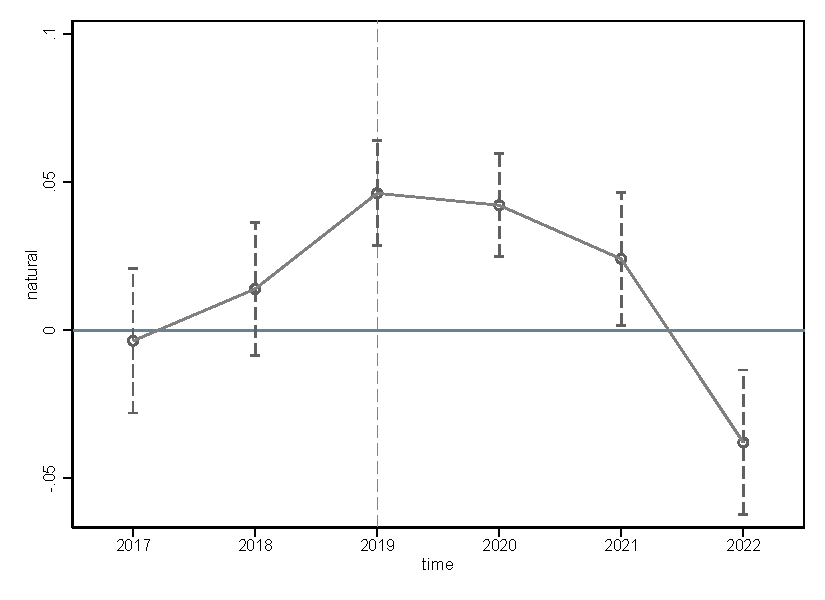
\includegraphics[width=0.5\textwidth]{../figures/did_1.pdf}\label{fig:did_income}}
    \hfill % Adds horizontal space between figures
    \subfloat[Effect to price concession]{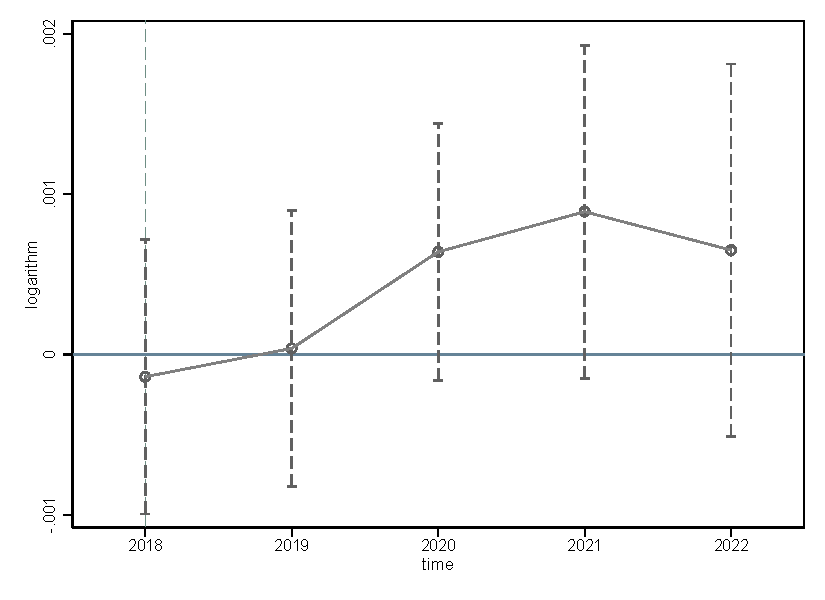
\includegraphics[width=0.5\textwidth]{../figures/did_2.pdf}\label{fig:did_price_concession}}
    \hfill % Adds horizontal space between figures
    \subfloat[Effect to number of house tours]{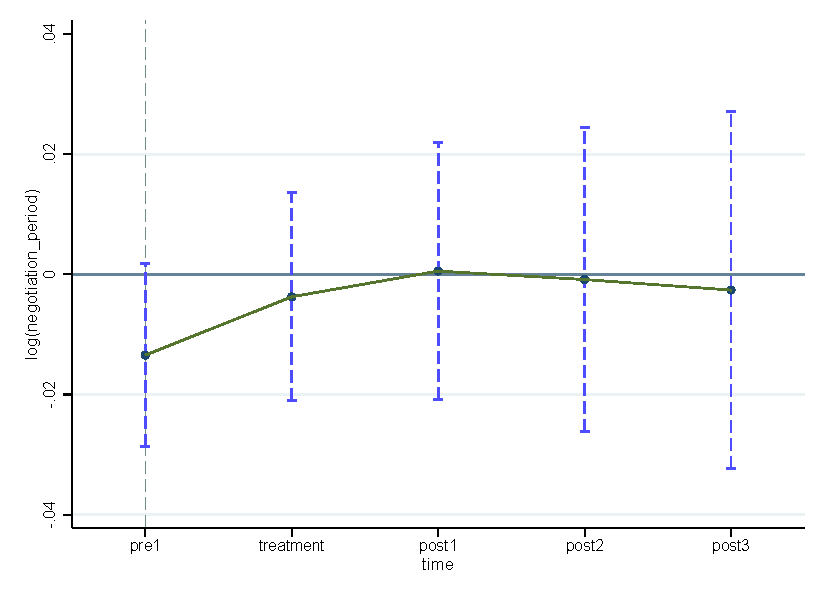
\includegraphics[width=0.5\textwidth]{../figures/did_3.pdf}\label{fig:did_lead_times}}
    \caption{Estimation of ACN Platformization Effect}
    \label{fig:dynamic_effect}
\end{figure}

The empirical findings elucidate that prior to the establishment of the ACN, there is an absence of discernible effects attributable to anticipation. Subsequent results for the fiscal year 2018 reveal that the ACN exerts a considerable influence on revenue generation, yet it manifests no significant impact on the metrics of price concessions and the number of house tours. This phenomenon indicates that the efficacy of the ACN model does not derive from an augmentation in client base through absorption but rather through the synthesis and integration of comprehensive data on the supply side. Post-2018 observations indicate the maturation of the platformization process, evidencing its expanding influence from the supply to the demand sector. Notably, a marked negative effect on price concessions is observed, underscoring the ACN's significant role in influencing consumer decision-making processes.

However, the years 2021 and 2022 witnessed a mitigated advantage of these factors due to the global epidemic, underscoring an imperative insight; despite the foundational establishment of online platformization, the inherent benefits of physical storefronts remain irreplaceable. This realization requires a re-evaluation of economic models, advocating a harmonious co-evolution of online and offline market paradigms. This strategic integration aims to leverage the unique strengths of each model to foster a more resilient and adaptive economic ecosystem.

\section{Conclusion and Discussion} \label{sec:conclusion}

The study of Lianjia's strategic expansion into China's real estate brokerage industry, particularly through the implementation of the ACN and the proliferation of offline branches, underscores a transformative impact on market dynamics and transaction efficiency. Our empirical research shows that Lianjia's approach, which seamlessly integrates online platforms with an extensive offline presence, significantly enhances revenue generation and influences consumer behavior, particularly through improved price concessions and increased home viewing. The study highlights the critical role of offline store information and community proximity in increasing transaction revenue and achieving market dominance, even in the face of increasing monopolization trends. Despite the adverse effects of the COVID-19 pandemic, which temporarily diluted the benefits of both customer base expansion and information dissemination, the resilience of physical stores emerges prominently. This resilience, coupled with the strategic leverage of online platforms, underscores the importance of a synergistic online-offline model in overcoming market challenges and maintaining competitive advantage. The findings argue for a nuanced understanding of platform-based monopolization in real estate, suggesting that the successful integration of digital and physical domains can significantly enhance service delivery, market penetration, and overall system competitiveness, paving the way for a more adaptive and robust market system in the face of evolving challenges.

%%%%%%%%%%%%%%%%%%%%%%%%%%%%%%%%%%%%%%%%%%%%%%%%%
\clearpage
\begin{singlespace}
%\bibliographystyle{plainnat}
%\bibliographystyle{chicago}
\bibliographystyle{aer}
\bibliography{our-cites.bib}
\end{singlespace}
%%%%%%%%%%%%%%%%%%%%%%%%%%%%%%%%%%%%%%%%%%%%%%%%%


%%%%%%%%%%%%%%%%%%%%%%%%%%%%%%%%%%%%%%%%%%%%%%%%%
%%%%% These commands start the appendix and change the Table & Figure numbering
\newpage
\appendix
\setcounter{table}{0}
\renewcommand{\tablename}{Appendix Table}
\renewcommand{\figurename}{Appendix Figure}
\renewcommand{\thetable}{A\arabic{table}}
\setcounter{figure}{0}
\renewcommand{\thefigure}{A\arabic{figure}}
%%%%%%%%%%%%%%%%%%%%%%%%%%%%%%%%%%%%%%%%%%%%%%%%%

% \section{Appendix Tables and Figures}
% \input{tab_tex/other-regressions.tex}


\end{document}


\subsection{Robustness Check} \label{subsec:robustness_check}


\begin{table}[H]
  \begin{center}
    \begin{scriptsize}
    \caption{Robustness Check Using HHI Index}
    \label{tab:sylized_fact}
    {
\def\sym#1{\ifmmode^{#1}\else\(^{#1}\)\fi}
\begin{tabular}{l*{6}{c}}
\toprule
            &\multicolumn{1}{c}{(1)}&\multicolumn{1}{c}{(2)}&\multicolumn{1}{c}{(3)}&\multicolumn{1}{c}{(4)}&\multicolumn{1}{c}{(5)}&\multicolumn{1}{c}{(6)}\\
            &\multicolumn{1}{c}{log(income)}&\multicolumn{1}{c}{log(income)}&\multicolumn{1}{c}{price concession}&\multicolumn{1}{c}{price concession}&\multicolumn{1}{c}{log(lead times)}&\multicolumn{1}{c}{log(lead times)}\\
\midrule
L.ln\_income &     -0.0864\sym{***}&      -0.108\sym{***}&                     &                     &                     &                     \\
            &   (0.00562)         &   (0.00684)         &                     &                     &                     &                     \\
\addlinespace
yearx2\_density&       0.726\sym{***}&       0.136\sym{***}&     0.00260         &    -0.00141         &      0.0300         &      0.0299         \\
            &     (0.110)         &    (0.0438)         &   (0.00446)         &   (0.00156)         &    (0.0847)         &    (0.0317)         \\
\addlinespace
yearx3\_density&       0.430\sym{***}&       0.106\sym{***}&     0.00651         &    -0.00190         &       0.238\sym{***}&      0.0571\sym{*}  \\
            &     (0.113)         &    (0.0396)         &   (0.00397)         &   (0.00149)         &    (0.0849)         &    (0.0297)         \\
\addlinespace
yearx4\_density&       0.281\sym{***}&      0.0229         &     0.00635\sym{*}  &   -0.000630         &       0.163\sym{*}  &      0.0182         \\
            &     (0.103)         &    (0.0399)         &   (0.00363)         &   (0.00143)         &    (0.0850)         &    (0.0303)         \\
\addlinespace
yearx5\_density&       0.220\sym{**} &      0.0420         &    0.000861         &    -0.00108         &       0.215\sym{***}&      0.0531\sym{*}  \\
            &    (0.0976)         &    (0.0418)         &   (0.00324)         &   (0.00136)         &    (0.0716)         &    (0.0304)         \\
\addlinespace
yearx6\_density&      -0.273\sym{**} &      -0.191\sym{***}&    -0.00421         &    -0.00590\sym{**} &      0.0668         &     0.00649         \\
            &     (0.134)         &    (0.0662)         &   (0.00466)         &   (0.00256)         &     (0.102)         &    (0.0480)         \\
\addlinespace
yearx7\_density&      -0.358\sym{***}&      -0.133\sym{*}  &    -0.00135         &    -0.00796\sym{***}&       0.148         &      0.0297         \\
            &     (0.131)         &    (0.0767)         &   (0.00506)         &   (0.00299)         &     (0.112)         &    (0.0604)         \\
\addlinespace
broker\_410  &     0.00129         &     0.00610\sym{*}  &   0.0000350         &   0.0000271         &    0.000518         &     0.00487\sym{**} \\
            &   (0.00128)         &   (0.00342)         & (0.0000461)         &  (0.000137)         &  (0.000952)         &   (0.00246)         \\
\addlinespace
ln\_end\_price&       0.898\sym{***}&       0.966\sym{***}&      0.0651\sym{***}&      0.0787\sym{***}&       0.241\sym{***}&       0.269\sym{***}\\
            &    (0.0366)         &    (0.0591)         &   (0.00248)         &   (0.00387)         &    (0.0294)         &    (0.0434)         \\
\addlinespace
ln\_watch\_people&      0.0605\sym{***}&      0.0636\sym{***}&     0.00194\sym{***}&     0.00153\sym{***}&       0.332\sym{***}&       0.315\sym{***}\\
            &   (0.00473)         &   (0.00666)         &  (0.000208)         &  (0.000272)         &   (0.00530)         &   (0.00676)         \\
\addlinespace
ln\_watch\_time&      0.0303\sym{***}&      0.0308\sym{***}&   -0.000105         &   -0.000319\sym{*}  &      0.0266\sym{***}&      0.0450\sym{***}\\
            &   (0.00300)         &   (0.00409)         &  (0.000123)         &  (0.000174)         &   (0.00263)         &   (0.00342)         \\
\addlinespace
ln\_nego\_changes&      0.0170\sym{**} &      0.0299\sym{**} &     0.00178\sym{***}&     0.00258\sym{***}&       0.134\sym{***}&       0.134\sym{***}\\
            &   (0.00806)         &    (0.0122)         &  (0.000289)         &  (0.000459)         &   (0.00870)         &    (0.0102)         \\
\addlinespace
ln\_negotiation\_period&      0.0606\sym{***}&      0.0575\sym{***}&    -0.00184\sym{***}&    -0.00182\sym{***}&       0.116\sym{***}&       0.143\sym{***}\\
            &   (0.00445)         &   (0.00680)         &  (0.000194)         &  (0.000301)         &   (0.00487)         &   (0.00668)         \\
\addlinespace
L.price\_concession&                     &                     &      -0.183\sym{***}&      -0.205\sym{***}&                     &                     \\
            &                     &                     &   (0.00582)         &   (0.00744)         &                     &                     \\
\addlinespace
L.ln\_lead   &                     &                     &                     &                     &      -0.112\sym{***}&      -0.120\sym{***}\\
            &                     &                     &                     &                     &   (0.00457)         &   (0.00605)         \\
\midrule
\(N\)       &       80476         &       45060         &       77780         &       43578         &       80476         &       45060         \\
R-squared   &       0.892         &       0.908         &       0.638         &       0.699         &       0.925         &       0.929         \\
\bottomrule
\multicolumn{7}{l}{\footnotesize Standard errors in parentheses}\\
\multicolumn{7}{l}{\footnotesize \sym{*} \(p<0.1\), \sym{**} \(p<0.05\), \sym{***} \(p<0.01\)}\\
\end{tabular}
}
  
  
    \end{scriptsize}
  \end{center}
\end{table}

\begin{table}[H]
  \begin{center}
    \begin{scriptsize}
    \caption{Robustness Check}
    \label{tab:sylized_fact}
    {
\def\sym#1{\ifmmode^{#1}\else\(^{#1}\)\fi}
\begin{tabular}{l*{4}{c}}
\toprule
            &\multicolumn{1}{c}{(1)}&\multicolumn{1}{c}{(2)}&\multicolumn{1}{c}{(3)}&\multicolumn{1}{c}{(4)}\\
            &\multicolumn{1}{c}{log(income) [lower]}&\multicolumn{1}{c}{log(income) [higher]}&\multicolumn{1}{c}{log(lead times) [lower]}&\multicolumn{1}{c}{log(lead times) [higher]}\\
\midrule
L.ln\_income &     -0.0529\sym{***}&     -0.0929\sym{***}&                     &                     \\
            &   (0.00594)         &   (0.00539)         &                     &                     \\
\addlinespace
yearx2\_density&       0.197\sym{***}&      0.0979\sym{*}  &      0.0260         &      0.0582         \\
            &    (0.0586)         &    (0.0502)         &    (0.0406)         &    (0.0373)         \\
\addlinespace
yearx3\_density&       0.207\sym{***}&      0.0242         &       0.129\sym{***}&      0.0224         \\
            &    (0.0483)         &    (0.0463)         &    (0.0345)         &    (0.0373)         \\
\addlinespace
yearx4\_density&       0.114\sym{**} &     -0.0313         &      0.0540\sym{*}  &      0.0282         \\
            &    (0.0453)         &    (0.0440)         &    (0.0318)         &    (0.0326)         \\
\addlinespace
yearx5\_density&       0.128\sym{***}&      0.0437         &      0.0250         &      0.0647\sym{*}  \\
            &    (0.0423)         &    (0.0492)         &    (0.0315)         &    (0.0330)         \\
\addlinespace
yearx6\_density&     -0.0765         &      -0.237\sym{***}&      0.0139         &     -0.0107         \\
            &    (0.0814)         &    (0.0805)         &    (0.0493)         &    (0.0565)         \\
\addlinespace
yearx7\_density&      -0.116         &      -0.103         &     -0.0161         &      0.0817         \\
            &    (0.0883)         &    (0.0872)         &    (0.0724)         &    (0.0774)         \\
\addlinespace
broker\_410  &     0.00416\sym{***}&   -0.000302         &    0.000511         &    0.000930         \\
            &   (0.00155)         &   (0.00142)         &   (0.00114)         &   (0.00110)         \\
\addlinespace
ln\_end\_price&       0.945\sym{***}&       0.928\sym{***}&       0.233\sym{***}&       0.255\sym{***}\\
            &    (0.0429)         &    (0.0409)         &    (0.0326)         &    (0.0322)         \\
\addlinespace
ln\_watch\_people&      0.0863\sym{***}&      0.0501\sym{***}&       0.327\sym{***}&       0.331\sym{***}\\
            &   (0.00529)         &   (0.00505)         &   (0.00550)         &   (0.00564)         \\
\addlinespace
ln\_watch\_time&      0.0282\sym{***}&      0.0327\sym{***}&      0.0309\sym{***}&      0.0334\sym{***}\\
            &   (0.00392)         &   (0.00310)         &   (0.00295)         &   (0.00276)         \\
\addlinespace
ln\_nego\_changes&      0.0259\sym{***}&      0.0200\sym{**} &       0.160\sym{***}&       0.110\sym{***}\\
            &   (0.00911)         &   (0.00886)         &   (0.00812)         &   (0.00901)         \\
\addlinespace
ln\_negotiation\_period&      0.0488\sym{***}&      0.0657\sym{***}&       0.123\sym{***}&       0.129\sym{***}\\
            &   (0.00517)         &   (0.00487)         &   (0.00487)         &   (0.00534)         \\
\addlinespace
L.ln\_lead   &                     &                     &     -0.0922\sym{***}&      -0.107\sym{***}\\
            &                     &                     &   (0.00461)         &   (0.00496)         \\
\midrule
\(N\)       &       66143         &       67756         &       66143         &       67756         \\
R-squared   &       0.883         &       0.897         &       0.917         &       0.927         \\
\bottomrule
\multicolumn{5}{l}{\footnotesize Standard errors in parentheses}\\
\multicolumn{5}{l}{\footnotesize \sym{*} \(p<0.1\), \sym{**} \(p<0.05\), \sym{***} \(p<0.01\)}\\
\end{tabular}
}
  
  
    \end{scriptsize}
  \end{center}
\end{table}

\newpage 
\section{Appendix One \label{sec:appendix:first}}
\renewcommand{\thetable}{B\arabic{table}}
\setcounter{table}{0}
\renewcommand{\thefigure}{B\arabic{figure}}
\setcounter{figure}{0}


% \input{fig_tex/fig_another_figure.tex}

\newpage
\section{Appendix Two
\label{sec:appendix:two}}
\renewcommand{\thetable}{C\arabic{table}}
\setcounter{table}{0}
\renewcommand{\thefigure}{C\arabic{figure}}
\setcounter{figure}{0}






When it comes to the estimation of the entry effect and its continuous effect, we use the following model:

\begin{equation}
  \begin{aligned}
    Y_{it} & = \beta_0 + \beta_1 Pre_3 + \beta_2 Pre_2 + \beta_3 Entry \\
    & + \beta_4 Post_1 + \beta_5 Post_2 + \beta_6 Post_3  + \bf{\alpha} \bf{X}_{it} + \tau_{it} + \mu_i + \epsilon_{it}.
  \end{aligned}
\end{equation}

where $Pre$ is the pre-period of lianjia's entry, $Entry$ is the entry period, and $Post$ is the post-period of lianjia's entry. All other model settings are the same as the previous model.

Finally, we construct a proxy variable to capture the continuous effect of the DBI. The model is as follows:

\begin{equation}
  \begin{aligned}
    Y_{it} & = \beta_0 + \beta_1 proxy\_entry + \beta_2 proxy\_pos\_1 \\
    & + \beta_3 proxy\_pos\_2 + \beta_4 proxy\_pos\_3 + \bf{\alpha} \bf{X}_{it} + \tau_{it} + \mu_i + \epsilon_{it}.
  \end{aligned}
\end{equation}

where $proxy\_entry$ is the product of the entry effect and the DBI, and $proxy\_pos\_i$ is the product of the post-period effect and the DBI. All other model settings are the same as the previous model. The results are shown in Appendix Table \ref{tab:Baseline} and Appendix Table \ref{tab:Dynamic}.

However, our estimates may not be asymptotically efficient due to the endogeneity of DBI and serial correlation issues. First, DBI is endogenous because the entry of lianjia is endogenous. This is due to the fact that lianjia will choose better locations with higher potential revenues in order to maximize profits. Second, the model suffers from serial correlation because our sample is during the boom period of China's real estate market, and as the number of transactions in the real estate market increases, so do the revenues and prices in the brokerage industry. In addition, lianjia tend to be concentrated in popular areas, which makes for greater growth and thus confounds our estimates. To solve this problem, we use a dynamic panel model for estimation. Dynamic panel models can capture the dynamics of the process by using the lagged dependent variable as a regression variable. This helps in understanding how the past values of the variables affect their current values. 

To estimate the dynamic panel model, we use the Arellano-Bond (1991) GMM estimator, which is a two-step estimator. The first step is to use the lagged dependent variable as an instrument for the current dependent variable, and the second step is to use the lagged residuals as an instrument for the current dependent variable. In this paper, we do not use system GMM estimator because the system GMM must assume that the lagged explanatory variables are independent of factors that do not vary over time in the region, and this clearly cannot hold in the present setting. The model is as follows: [\textbf{this should be a line that describes what measures that we use to construct the model}]

\begin{equation}
  \begin{aligned}
    \Delta Y_{it} & = \rho \Delta Y_{it-1} + \beta_1 \Delta Measure_{it} + \bf{\alpha} \Delta \bf{X}_{it} + \Delta \tau_{it} + \Delta \epsilon_{it}.
  \end{aligned}
\end{equation}

where $\Delta Y_{it}$ is the first difference of the dependent variable, $\Delta Measure_{it}$ is the first difference of the our three measurement methods, $\Delta \bf{X}_{it}$ is the first difference of the control variables, $\Delta \tau_{it}$ is the first difference of the time dummy variable interacting with the fixed effect of the business area, and $\Delta \epsilon_{it}$ is the first difference of the error term. The standard errors are clustered at the individual level. The results are shown in Appendix Table \ref{tab:GMM}.


For Table \ref{tab:Baseline}, the result reveals a significant correlation between the lianjia's local market power and lianjia's income in this given community. However, we discovered no substantial influence of lianjia's local market power on the housing prices or transaction periods in the same community. This could be interpreted to mean that whilst Lianjia's local market power could induce an increase in income, it does not necessarily grant them any significant pricing power nor expedite the transaction period. Therefore, we may deduce that the augmentation of Lianjia's income is primarily driven by an increase in the number of transactions, presumably due to more property listings by Lianjia within the community. This suggests that although lianjia can control more market share in the local market, it does not necessarily mean that it can have monopoly power in this given region. This is partially because the price of the house is determined by the market, and there are also some potential other brokerages that can enter the market. However, lianjia's local market power can still have a significant influence on the income because they can list more housings and have more transactions in the local market.

To further test the results, we first check if lianjia's entry effect and continuous effect is significant. For column 1, 3, and 5 of the Table \ref{tab:Dynamic}, the result reveals that before the lianjia's entry, the natural logarithm of income, housing price and transaction period are not significant. After the entry, we see that after lianjia's entry into this local market, lianjia can immediately increase their income and keep making significantly more income comparing with previous periods. Besides, we see that the entry do not significantly increase the housing price immediately but significantly increase housing price one year after but later on turning back to the normal pricing. Lastly, the lianjia's entry do not significantly lowers the transaction periods. This is consistent with our previous results that lianjia's entry can significantly increase the income but not the housing price and transaction periods in equilibrium.

Lastly, we use the third measurement to test after the lianjia's entry, the continuous effect of lianjia's local power of the local market. For column 2, 4, and 6 of the Table \ref{tab:Dynamic}, the result reveals that the continuous effect of lianjia's local power of the local market is significant for the income, housing price and transaction periods. This result indicates that in different period, the lianjia's local market power can have different influence on the market.

